\section{Introduction}\label{introduction}


Large scale real-world systems are typically modelled in the form of graphs.
Consequently, A large number of applications require processing graph data which contains rich relational information between different entities (e.g., online social media, disease outbreaks, recommendation engines, knowledge graphs and navigation systems).
Deep Learning and more precisely Convolutional Neural Networks have shown tremendous performance over non-graph data such as images by capturing the spatial relation between pixels of image and extracting features over multiple layers.
However, this machine learning scheme has shown its limits for graph data and the learning on such data is still challenging~\cite{zhou2018graph}.
Indeed, the models have to capture the connections in the data while ensuring invariance of graph data representation, even without fixed ordering between the nodes (i.e., the adjacency matrix representing the connections between nodes varies but still results in the same graph). %different
To overcome this limitation, the graph data is passed through embedding algorithms which map the large graphs to lower dimensions which are then used for downstream processing with GNNs.
Graph embedding algorithms enable models operating on low dimensional euclidean datasets (i.e., such as images) to graph data by mapping them into a low dimensional embedding.
%Traditional Deep Neural Networks fail to capture the nuances of structured data but a specific class of algorithms, namely, Graph Neural Networks (GNNs) have shown state of the art performance on such complex graph data for node classification, link prediction etc.
%An important pre-processing step for using graph data with machine learning is embedding the high dimensional graph data to a low dimensional representation for easy processing by machine learning algorithms.
In many applications, such embeddings are released for further processing to save storage cost without considering the privacy implications.

Large graph dataset raises the question of privacy specifically if the algorithms and models are trained with private and potentially sensitive data.
Consider a graph capturing the outbreak of a disease where the nodes represent the individuals, medical symptoms as the node features and the edges indicating the disease transmission.
Typically, in such datasets a GNN provides state of the art performance for predicting disease for an arbitrary user in the graph (node classification) and determining the future outbreak (link prediction).
For such embedding models which do not account privacy, an adversary can however infer the health status of a particular user (node in graph) by identifying whether the user was part of the training data or not.
Further, the adversary can potentially reconstruct the sensitive graph input from the low dimensional embeddings. % enabling the adversary to extract the sensitive input to the models.
Finally, graph embeddings capture important semantics from the input graph while maintaining the contextual information in the form of preferential connection which can be exploited to infer sensitive attributes about an individual.
These three privacy attacks, namely, membership inference, graph reconstruction and attribute inference, are examples of a direct privacy violation of the individual which can further be used without user consent. % for deciding medical insurance premium or job hiring.
Further, companies spend enormous resources to annotate the training dataset to achieve state of the art performance and such attacks inferring training data also violates the Intellectual Property.
%Hence, studying and mitigating privacy risks is crucial specifically with the onset of data protection laws such as HIPAA and GDPR.

%In the context of Machine Learning (ML), a privacy violation occurs when an adversary infers something about a \textit{particular} user's data record in the training dataset which cannot be inferred from other models trained on similar data distribution~\cite{membershipinf,whitebox}.
%This information leakage is quantified using the success of inference attacks. %: membership inference, attribute inference and reconstruction attacks.
%In attribute inference attacks, the attacker infers sensitive features of an individual's data record used in model's training.
%A stronger case of attribute inference is where the attacker reconstructs a portion of the sensitive training data itself, i.e, data reconstruction attack.
%In case of membership inference, the adversary traces a particular individual's record to the training dataset, i.e., identify whether a given data record was a member of the training data.

Prior literature in privacy attacks focus on models trained on non-graph data including text, images and speech to study the vulnerability to membership inference~\cite{ndss19salem,membershipinf}, attribute inference~\cite{attributeinf,attributeinf2}, property inference~\cite{propertyinf}, model inversion~\cite{modelinversion} attacks as well as model parameter and hyperparameter stealing attacks~\cite{timing,stealml,8418595}.
While well studied in traditional ML, the privacy risk in graph-based ML models under adversarial setting has not been fully explored and quantified. % is not fully explored.

%In this work, we evaluate the vulnerability of graph embedding algorithms against the threat from three privacy attacks: membership inference, graph reconstruction and attribute inference.

\section{Contribution and Key Results}
\label{contribution}

In this work, we propose the first comprehensive privacy analysis of Graph Embedding algorithms under different threat models and adversary assumptions.
We mainly focus on exploiting publicly released graph embeddings trained with private data, used for different downstream tasks, under various practical attacks which violates the user's data privacy: membership inference, graph reconstruction and attribute inference.

\begin{figure}[!htb]
\centering
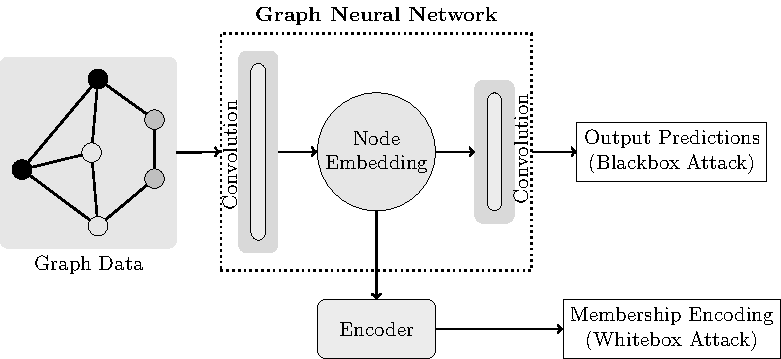
\includegraphics[width=0.6\linewidth]{./figures/Attacks/MIA.pdf}
%\caption{Blackbox and Whitebox Inference attacks to distinguish between members and non-members of $G_{train}$.}
\caption{Blackbox and whitebox inference attacks to distinguish members and non-members of the training graph.}
\label{mia}
%\vspace{-2mm}
\end{figure}

First, we evaluate the privacy leakage under membership inference attacks where the gaol of the adversary is to infer whether a given user's node was used in the training graph dataset or not.
This is a binary classification problem where the adversary learns the threshold to predict the membership of a user node.
Depending on the adversary's knowledge, we consider two settings: blackbox (with and without auxiliary knowledge) and whitebox.
As shown Figure~\ref{mia}, to distinguish between members and non-members of the training graph, the blackbox attacks exploit the statistical difference in output predictions while the whitebox attack exploits the intermediate low dimensional embedding.
The blackbox setting considers the specific case of downstream node classification task for convolution kernel based graph embedding with neural network. % (we consider the embeddings from four different architectures of GNNs: GCN~\cite{Kipf2016tc}, GraphSAGE~\cite{NIPS20176703}, GAT~\cite{velickovic2018graph}, and TAGCN~\cite{du2018topology}). 
In this setting, we propose two attacks for membership inference: with auxilary knowledge on the data distribution (shadow model attack) and without auxilary knowledge (confidence score attack).
Here, we show that the proposed attacks have an inference accuracy of 78\%, 63\%, and 60\% for confidence score attack and 62\%, 60\%, and 55\% for shadow model attack, respectively for three standard benchmarking datasets, i.e., Cora, Citesser and Pubmed dataset.
For the whitebox setting, we propose an unsupervised attack for the more generic case of using just the graph embeddings to differentiate whether a given node was part of the training graph or not.
We show that an adversary in this setting can predict the training data with a high accuracy (70\% on average on the three datasets).

\begin{figure}[!htb]
    \centering
%    \begin{minipage}[b]{1\linewidth}
%    \centering

    \subfigure[Adversary trains attack model on auxiliary subgraph]{
   	\label{fig:mem_soft_label}
    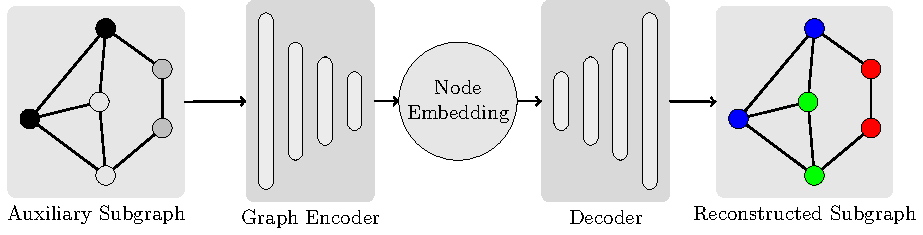
\includegraphics[width=0.65\linewidth]{./figures/Attacks/reconstruction.pdf}
    }
%\hspace{4mm}
    \subfigure[Attack model reconstructs target graph]{
    \label{fig:mem_soft_label}
    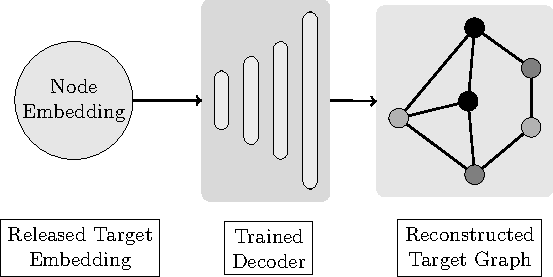
\includegraphics[width=0.45\linewidth]{./figures/Attacks/reconstruction2.pdf}
    }
%    \end{minipage}
%\vspace{-2mm}
    \caption{Attack methodology for graph reconstruction from released embeddings.}
    \label{fig:recattack}
%\vspace{-1mm}
\end{figure}

Second, we propose a novel graph reconstruction attack where the adversary, given access to the node embeddings of a subgraph, trains an encoder-decoder model to reconstruct the target graph from its publicly released embeddings (Figure~\ref{fig:recattack}).
This attack has serious privacy implications since the adversary reconstructs the input graph dataset which can be potentially sensitive.
The proposed attack has high precision: 0.722 for Cora, 0.778 for Citeseer and 0.95 for Pubmed dataset.
Moreover, on increasing the adversary's prior knowledge, the attack performance increases significantly.
An important privacy implication is link inference, i.e, predicting whether there exists a link between any two nodes in the graph.
Through this attack, an adversary infers a link between nodes with 93\%, 90\% and 57\% of accuracy for respectively Cora, Citeseer and Pubmed dataset, compared to the 50\% baseline random guess accuracy.




Finally, we propose the attribute inference attack where the adversary tries to infer sensitive attributes for user node in the graph using the released graph embeddings.
We consider two state of the art unsupervised random walk based embeddings, Node2Vec~\cite{node2vec} and DeepWalk~\cite{deepwalk}, on two real-world social networking datasets: Facebook~\footnote{http://snap.stanford.edu/data/ego-Facebook.html} and LastFM~\footnote{http://snap.stanford.edu/data/feather-lastfm-social.html}, where the adversary aims to infer the user gender and location, respectively.
Given access to the embeddings of a subgraph and corresponding sensitive attributes, we model attribute inference as a supervised learning problem.
The adversary trains a supervised attack model to predict sensitive hidden attributes for target users given the released publicly available target embeddings.
Here, the attack model's F1 score (capturing the balance between precision and recall) on LastFM was as high as 0.65 for DeepWalk and 0.83 for Node2Vec.
For Facebook, the F1 score was 0.61 for Node2Vec and 0.59 for DeepWalk.

The extended version of our analysis is available in preprint~\cite{hal-02956397}.
%A longeur version of this extended abstract is available~\cite{hal-02956397}.
In addition, the code for all the experiments is made publicly available for easy reproducibility\footnote{\url{https://github.com/vasishtduddu/GraphLeaks}}.


\section{Discussions and Conclusions}
\label{conclusion}


This work provides the first comprehensive privacy risk analysis related to graph embedding algorithms trained on sensitive graph data.
Specifically, we quantify privacy leakage of three major classes of privacy attacks under practical adversary assumptions and threat models, namely membership inference, graph reconstruction and attribute inference.
%Firstly, an adversary conducting a membership inference attack aims to infer whether a given user's node was used in the training graph dataset or not.
%Secondly, publicly released embeddings can be inverted to obtain the input graph data enabling an adversary to perform graph reconstruction attack on the sensitive graph data.
%This further enables the adversary to perform link inference attack to infer whether a link exists between two nodes in the network.
%Finally, we show that an adversary can infer sensitive hidden attributes of users such as gender and location from the graph embeddings.
Our results underlines many privacy risks in graph embeddings and calls for further research to mitigate these privacy threats.


Potential mitigation strategies to lower the privacy risks can be considered.
For instance, lowering the precision of the embedding vector for each node by rounding can help to reduce the attack model from learning rich features about the inputs~\cite{membershipinf,nlp}.
In the proposed attacks, the attacker model is a machine learning algorithm vulnerable to adversarial examples, i.e, imperceptible noise added to the output prediction to force the target model to misclassify.
The embeddings can be released with an additional adversarial noise to misclassify the target model while additionally ensuring utility~\cite{attriguard,memguard}.
Further, the inference attacks can be modelled within the training process as a minimax adversarial training with joint optimization to minimize the model loss using the graph embeddings (e.g., GNNs) while maximising the adversary's loss on inferring the sensitive inputs~\cite{advreg,textembleak}.
Finally, Differential Privacy can provide a theoretical bound on the total privacy leakage from the downstream processing from embeddings on an individual's data point~\cite{dptext,dpne}.
However, the efficacy of these potential mitigations are left for future work.








